\documentclass[12pt, a4paper]{article}
\usepackage[margin=1.5cm]{geometry}
\usepackage{graphicx} 
\usepackage{tikz}
\usepackage{hyperref}
\usepackage{mathptmx}
\usepackage{fancyvrb}


\usetikzlibrary{calc}
\AddToHook{shipout/background}{%
    \begin{tikzpicture}[remember picture, overlay]
        \draw[black, thin, rounded corners=10pt] ($(current page.north west)+(1cm,-1cm)$) 
            rectangle ($(current page.south east)+(-1cm,1cm)$);
    \end{tikzpicture}%
}




\begin{document}
\noindent\textbf{Date: }30 July, 2025
\\
\textbf{Experiment No.: }2
\\
\textbf{Experiment Name.: }Implementation of basic signal in MATLAB
\\
\textbf{Theory: } \\
Signals and systems form the foundation of many engineering applications. In this lab, we examined fundamental continuous-time signals: the unit step, unit impulse, ramp, and sinusoidal signals. These signals are building blocks for more complex waveforms and are essential in analyzing system behavior. The unit step represents sudden changes, the impulse models instantaneous events, the ramp shows linear growth, and the sine wave demonstrates periodic oscillations. Understanding these signals helps in characterizing system responses in both time and frequency domains.
\\ \textbf{Code: }
\begin{Verbatim}
clear all;
close all;
clc;
f=50;
t = -10:1:10;
signals = {(t >= 0), (t == 0), t.*(t >= 0), 20*sin(30*pi*f*t)};
titles = {'Step', 'Impulse', 'Ramp', 'Sine'};
j = 1;
for i = 1:4
subplot(4,2,j);
plot(t,signals{i},'k');
title([titles{i},' (Continuous)'],'FontSize', 20);
xlabel('t','FontSize', 18);
ylabel('u(t)','FontSize', 18);
subplot(4,2,j+1);
stem(t,signals{i},'k');
title([titles{i},' (Discrete)'],'FontSize', 20)
xlabel('n','FontSize', 18);
ylabel('u(n)','FontSize', 18);
j=j+2;
end
\end{Verbatim}
\textbf{Result: }
\begin{figure}[h]
    \centering
    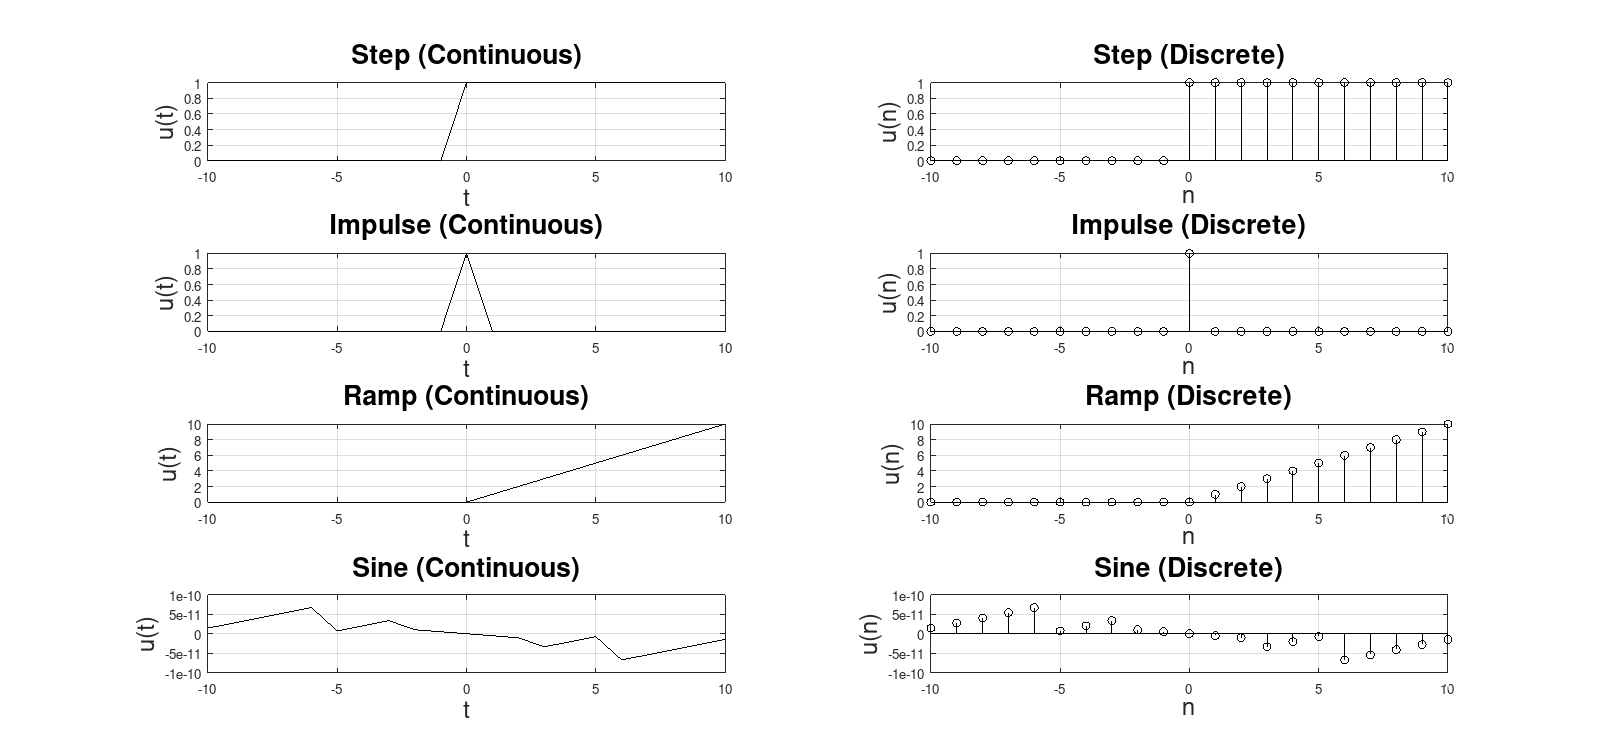
\includegraphics[width=0.9\linewidth]{plots.png}
    \caption{Basic Signals}
    \label{fig:placeholder}
\end{figure}



\noindent \textbf{Discussion: }\\
The lab involved generating and visualizing these signals using MATLAB. The unit step and
impulse signals were approximated using logical conditions, while the ramp and sine signals
required element-wise and scalar operations, respectively. The plots demonstrated how each
signal behaves over time, with the step function transitioning abruptly, the impulse appearing
as a single spike, the ramp increasing linearly, and the sine wave oscillating periodically. The
use of plot() and stem() helped distinguish between continuous and discrete representations.
Challenges included correctly scaling the sine wave’s frequency and ensuring proper indexing
for plotting.
\vspace{10pt}

\noindent \textbf{Conclusion:}\\
This lab successfully demonstrated the generation and analysis of basic continuous-time
signals. The exercises reinforced the importance of signal properties such as amplitude,
frequency, and time-shifting. By comparing continuous (plot) and discrete (stem)
representations, we observed how signals can be interpreted differently based on their
domain. These concepts are crucial for advanced topics in signal processing, control systems,
and communications. 
\end{document}
